\begin{abstract}
Im Rahmen des Serious Games Praktikums wurde \textit{BunnySuite} entwickelt, ein Benchmark-Framework für 2D-Grafik-Bibliotheken. Es besteht aus einer grafischen Benutzeroberfläche sowie den Implementierungen für die vier Bibliotheken Kha, LibGDX, SDL und XNA/Monogame. Die Tests werden in der GUI definiert und anschließend vollautomatisch durchgeführt. Die Ergebnisse werden grafisch in Diagrammen aufbereitet. Die Testergebnisse zeigen, dass die Leistungsfähigkeit der getesteten Bibliotheken in verschiedenen Bereichen sehr unterschiedlich sind. Dadurch, dass \textit{BunnySuite} diese Unterschiede transparent macht, können Entwickler leichter die für ihren Zweck beste Bibliothek finden. Außerdem helfen die Ergebnisse den Entwicklern der Bibliotheken bei der Optimierung der Performance.
\end{abstract}

\chapter{Einleitung}
Moderne Computerspiele setzen meistens auf eine graphische Darstellung ihrer Spielwelt. Dabei geht, vor allem in den letzten Jahren, der Trend verstärkt in die Richtung fotorealistischer 3D-Renderings und weg von der simpleren 2D-Darstellung.
Dabei ist schnelles 2D-Rendering immer noch eine nichttriviale Aufgabe für GPUs. Für viele Anwendungen sind die verfügbaren Bibliotheken im Allgemeinen immer noch viel zu langsam. Um das zu verbessern, haben wir mit \textit{BunnySuite} ein Framework entwickelt, mit dem gängige 2D-Grafik-Bibliotheken einem automatisierten Stresstest ausgesetzt werden können.\\
Mit dem \textit{BunnyMark}, entwickelt von Iain Lobb\footnote{\url{http://blog.iainlobb.com/2010/11/display-list-vs-blitting-results.html}}, gab es bereits eine Metrik zum Vergleich von Bibliotheken. Jedoch wurde hier nur die Anzahl der gerenderten Objekte (in diesem Fall Häschen, deshalb der Name) gemessen, bei denen noch 60 fps erreicht werden. Diese Zahl war nur schwer zu interpretieren und musste für ein ausführlicheres Ranking durch die aussagekräftigere Metrik  \textit{Renderzeit pro Frame bei X Objekten} ersetzt werden. Auch findet diese Messung bei BunnyMark zu Demozwecken nur interaktiv statt: Häschen werden per Mausklick zur Szene hinzugefügt. Im von uns entwickelten BunnySuite-Framework können solche Messungen automatisiert erfolgen. Die Tests für mehrere Frameworks werden automatisch nacheinander gestartet und das Ergebnis wird in zwei Diagrammen zusammengefasst. Das Framework ist leicht erweiterbar, so dass man es mit wenig Aufwand an neue Bibliotheken anpassen kann.\\
Das vollautomatisierte Test-Framework soll Entscheidern bei der Spieleentwicklung die Möglichkeit eines Rankings bieten, um die richtige Bibliothek für ihre Anforderungen zu finden. Desweiteren sollen Entwickler von Bibliotheken das Framework nutzen können, um ihre eigene Bibliothek zu testen und zu optimieren. Die Leistungen der Bibliotheken können so transparent verglichen werden, was den Wettbewerb zwischen ihnen stimulieren und Anreize setzen soll, stärker an der Performanz zu arbeiten.\\
Im folgenden Kapitel wird zunächst kurz der Projektplan aufgeführt (Kapitel \ref{ch:projektplan}) und anschließend werden die Grundlagen von 2D-Grafik-Libraries und Benchmarking beschrieben (Kapitel \ref{ch:basics}). Im Hauptteil der Ausarbeitung werden das grundlegende Konzept (Kapitel \ref{ch:konzept}) und einige Aspekte der praktischen Umsetzung des entwickelten Frameworks (Kapitel \ref{ch:umsetzung}) vorgestellt. Danach gehen wir in Kapitel \ref{ch:results} auf ein paar interessante Testergebnisse ein. Im letzten Kapitel wird die Arbeit zusammengefasst und es werden einige Erweiterungsmöglichkeiten genannt.

\chapter{Zeitplan und Aufgabenverteilung}
\label{ch:projektplan}
Das Team hat sich darauf geeinigt, dass jeder Entwickler sich auf eine Bibliothek konzentriert. In regelmäßigen Meetings werden Konzepte diskutiert und Designentscheidungen getroffen. Auf diese Weise soll in allem Frameworks eine vergleichbare Implementierung erreicht werden.\\
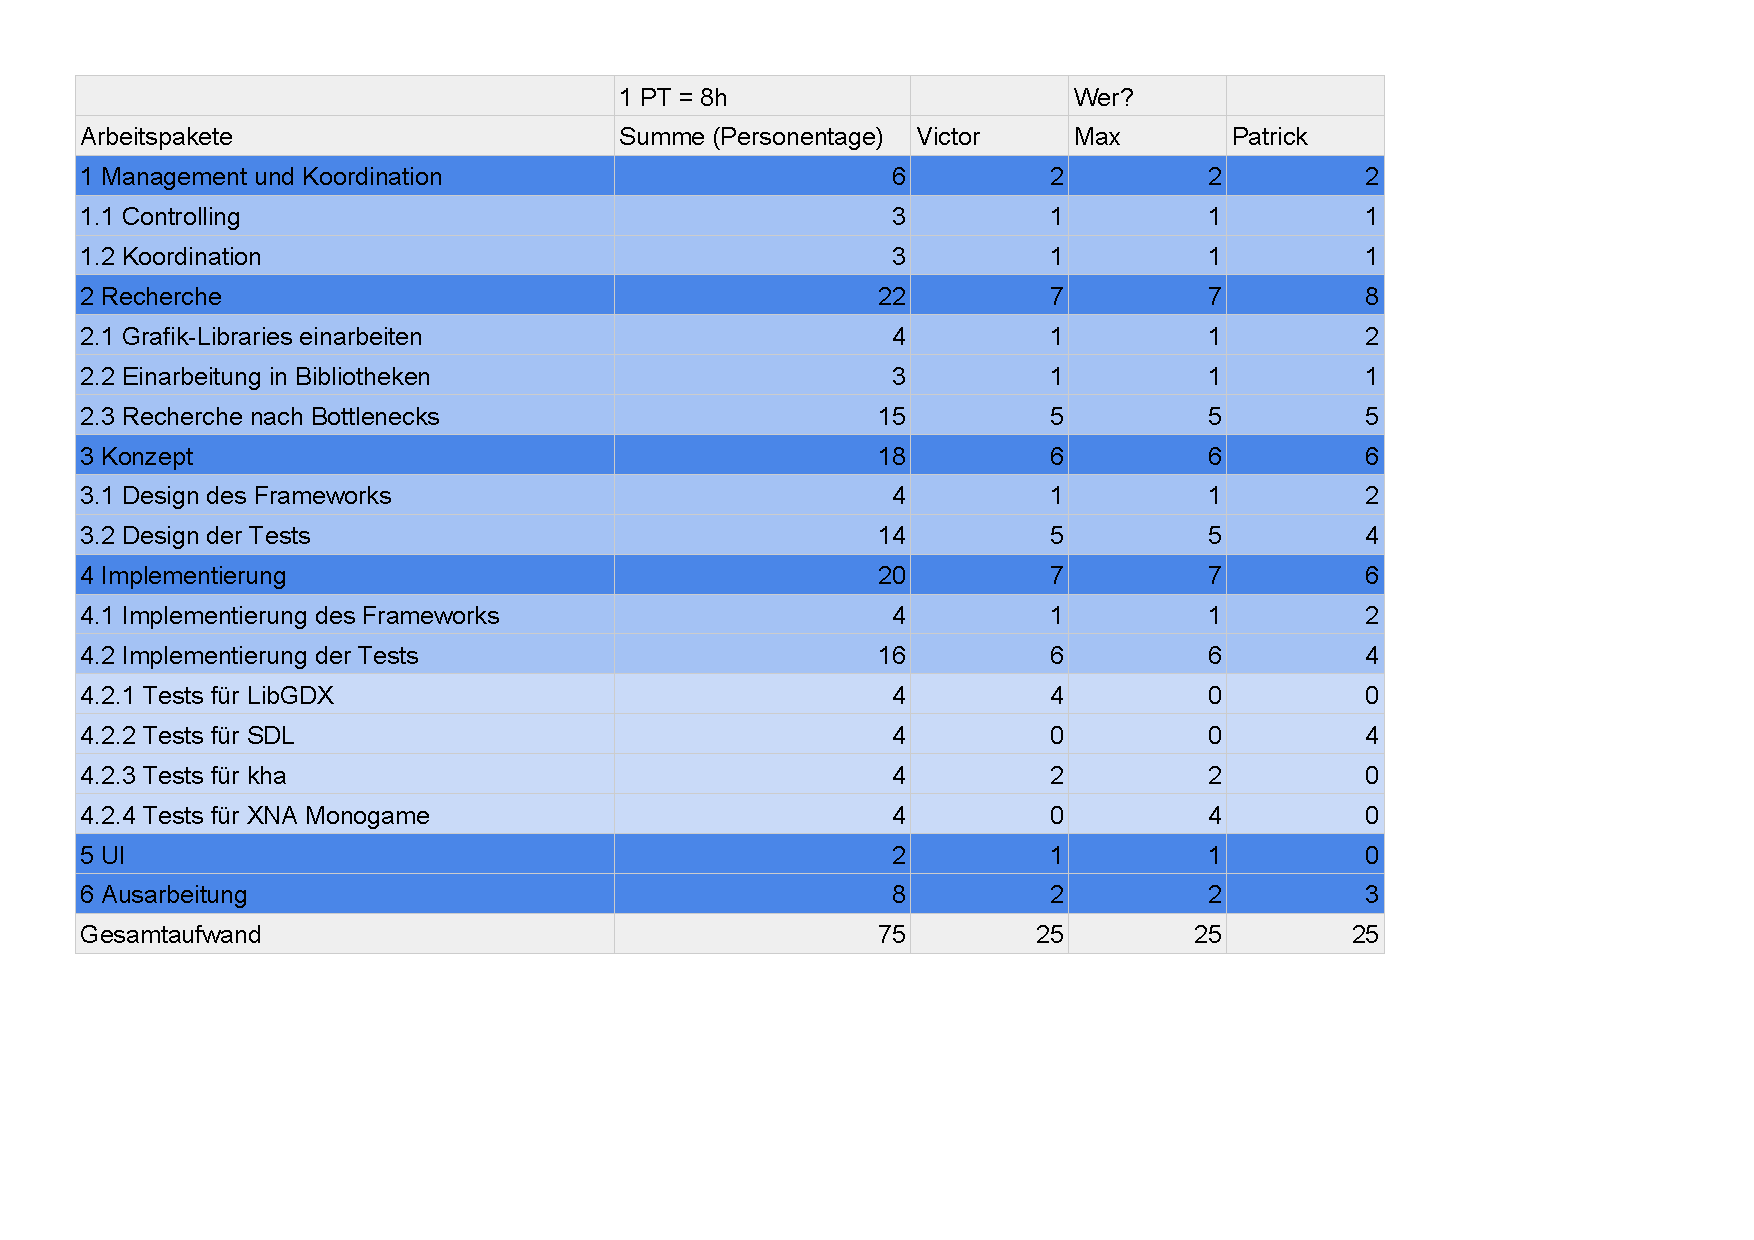
\includegraphics[width=1.2\textwidth]{projektplan.pdf}


\chapter{Grundlagen}
\label{ch:basics}
\section{2D-Frameworks}
Game-Frameworks sollen die Entwickler beim Implementieren der Game-Loop unterstützen. Diese Game-Loop besteht hauptsächlich aus 2 Phasen:

\begin{description}
\item[Update()] Der interne Zustand der Spielwelt und ihrer Objekte wird aktualisiert, beispielsweise die Position der Spielfigur gemäß der Benutzereingaben angepasst oder das nächste Frame in einer Animation wird ausgewählt oder die Punktzahl erhöht. Zeitgleich finden hier auch komplexere Berechnungen statt, wie die Kollisionsbestimmung, die wieder zu neuen Berechnungen führen kann (Positionen werden angepasst, damit Objekte sich nicht überlagern; "Gesundheitswerte" werden bei Treffern verringert).\\
\item[Draw()] Die im vorherigen Schritt berechnete Spielwelt wird auf dem Bildschirm dargestellt. Dazu gehören die korrekte Position aller Objekte, die Texturierung und Beleuchtung dieser Objekte, und gegebenenfalls Transformationen (Skalierung, Rotation). Auch muss bei Überlagerung von Objekten auf die korrekte Darstellung geachtet werden. Dies gilt auch für verdeckte Rückseiten von Objekten. Anschließend wird noch die Benutzeroberfläche über den Bildschirminhalt gelegt.\\
\end{description}

Die Game-Frameworks unterstützen die Entwickler, indem sie verschiedene Funktionalitäten bereits für die jeweilige Zielplatform optimiert zur Verfügung stellen. Dazu gehören:

\begin{itemize}
\item Einfacher Zugriff auf Eingabegeräte. Das können einfach Maus und Tastatur sein, aber auch plattformspezifische Gamepads oder auch Touch- und Gestensteuerung, vor allem für VR.\\
\item optimierte Klassen für Assets. Dazu gehören Audiodateien, die gestreamt werden, oder auch Texturen, die möglichst effizient für den Grafikspeicher komprimiert werden.\\
\item optimierte Renderfunktionen, die direkt Grafikschnittstellen wie OpenGL, Direct3D oder Vulkan ansprechen. Diese können auch bereits Transformationen wie Drehungen oder Einfärbungen anbieten. Diese können direkt 3D-Meshes, Bilder/Texturen, Text oder auch Primitive wie Dreiecke oder Rechtecke darstellen.\\
\end{itemize}

Diese Bibliotheken helfen den Entwicklern, eine effiziente Implementierung zu erreichen, ohne sehr hardwarenahe Optimierungen selber programmieren zu müssen. Somit soll sehr einfach der "Goldstandard" von 60 Frames per Second in der Darstellungen erreicht werden, bei dem für jede Iteration der Gameloop eine Rechenzeit von knapp 16,67 ms zur Verfügung steht. Dies beinhaltet das Einlesen von Assets wie Texturen vom Speichersystem der jeweiligen Plattform, was bereits für Verzögerungen sorgen kann.\\ 
Der wahrscheinlich größte Unterschied zu 3D-Frameworks besteht in der Komplexität der Grafikberechnung. So muss das 2D-Framework keine Informationen über Oberflächen der Objekte, z.B. Oberflächenorientierung zu Lichtquellen über NormalMaps oder Materialeigenschaften für das \emph{Physically Based Rendering (PBR)}, außer der konkreten Farbe, kennen.\\
Auch können diese Objekte bereits ihrer Darstellung entsprechend als Sprite vorliegen, die gegebenenfalls noch mit Transformationen wie Skalierung an die jeweilige Situation  angepasst, direkt dargestellt werden können. Somit muss kein komplexes dreidimensionales Objekt auf einmal im Speicher gehalten werden, bei dem man sowieso nur die der Kamera zugewandten Seite sieht, sondern nur ein Spritesheet mit den möglichen Orientierungen und Bewegungsphasen des Objekts.
Ebenso entfällt bei der Darstellung eine komplexe Berechnung der Überlagerung oder verdeckter Rückseiten der Objekte. Es wird nur die momentane Orientierung der Objekte dargestellt. Die Verdeckung von Objekten kann durch layerbasiertes Rendering gelöst werden:
\begin{enumerate}
\item Hintergrund rendern\\
\item Nicht Spieler Objekte rendern\\
\item Spieler Objekt rendern\\
\item Benutzeroberfläche rendern\\
\end{enumerate}
Diese Besonderheiten vereinfachen die Berechnung im 2D-Darstellungsfall. Dadurch ist dieser Fall aber nicht so gut optimiert, wie die 3D-Anwendung, und es werden regelmäßig Grenzen ausgereizt.\\
\\
Diese Problematik hat konkrete Auswirkungen auf den Ablauf von Videospielen. Hier das Beispiel des Speedrunnings:

Beim Speedrunning versucht der Spieler, so schnell wie möglich die Zielbedingung zu erfüllen. Das sind, je nach Spiel und Kategorie, das einsammeln aller Collectibles im Spiel, das Besiegen des \mbox{Endgegners} oder aber "nur" das Erreichen der Credits nach dem Spiel. Aus mehreren Gründen sind diese Spieler an einer guten Perfomanz des Spieles interessiert:

\begin{itemize}
\item Die Rekorde im selben Run (selbes Spiel, selbe Kategorie) sind oft nur Sekundenbruchteile schneller als die zweitschnellsten Ergebnisse.
\item Zum Erreichen des Zieles dürfen, abhängig von der Kategorie, auch Spielfehler ausgenutzt werden, oder sogar durch Speichermanipulation und gezielten Over/Underflows das Spiel umgeschrieben werden. Hierfür sind oft pixelgenaue Positionierung in der Spielwelt und auf den Frame perfekte Benutzereingaben notwendig, um diese "Glitches" gezielt ausführen zu können.
\end{itemize}

Jeglicher Performance-Einbruch des Spieles erschwert die Jagd auf den nächsten Weltrekord. Die einfachste Lösung dieses Problems ist es, das Spiel auf immer stärkeren Rechnern zu starten. Fehlende Optimierung des Spiels wird durch mehr Rechenleistung ausgeglichen.
Dies ist aber nicht immer möglich, vor allem bei Spielen, die nur auf Konsolen laufen. Hier muss der Speedrunner die fehlende Optimierung selber ausgleichen. Zum Beispiel:
\begin{itemize}
\item Betrachten des leeren Himmels: Es werden keine Objekte auf dem Bildschirm dargestellt - \emph{Daggerfall, PC Speedrun}
\item Das gezielte zerstören von bestimmten Gegnern: Es werden weniger Objekte auf dem Bildschirm dargestellt - \emph{Mega Man 3, NES }
\end{itemize}
Dies sind auch erste Ansätze für die Sektion \nameref{sec:bottlenecks}.

\section{Benchmarking}
Um eine möglichst einfache Bedienung zu gewährleisten, soll der Benchmark vollautomatisiert erfolgen. Wichtigste Eigenschaft des Benchmarks ist die Vergleichbarkeit der Ergebnisse. Dazu wurde die \textit{Renderzeit pro Frame bei X Objekten} als Kennzahl eingeführt. Wie bei allen empirischen Untersuchungen muss diese den folgenden drei Kriterien genügen\footnote{Siehe: \url{http://www.uni-leipzig.de/~emkf/Referate/G\%C3\%BCtekriterien\%20PPT.pdf}}:\\
\begin{description}
\item[Validität] Dass sich die Kennzahl mit empirischen Messergebnissen deckt, ist garantiert, da sie empirisch zustande kommt. Es wurde die in Entwicklerkreisen übliche Größe {\em Renderzeit pro Frame in Sekunden} gewählt. Die Inverse dieser Größe, {\em Frames per Second}, ist zwar bei Nutzern und Marketing sehr beliebt, nicht jedoch bei technischen Entwicklern, unserer Zielgruppe. Ein arbiträres Punktesystem würde die Messwerte nur unnötig verschleiern und den Eigenschaften eines guten Benchmarks widersprechen.\\

\item[Objektivität] ist durch die Wohldefiniertheit der einzelnen Testverfahren gegeben (siehe \ref{sec:tests}). Die Implementierung in den einzelnen Frameworks soll möglichst gleich sein. Somit sind die verschiedenen Messwerte auf dem selben Computer nur auf die Effizienz der verwendeten Bibliothek zurückzuführen und nicht auf die Implementierung der Tests durch den verantwortlichen Entwickler.\\
Die BunnySuite soll speziell die Grafikleistung der verschiedenen Frameworks bewerten. Daher muss gewährleistet sein, dass das Testergebnis nicht maßgeblich von Berechnungen auf der CPU beeinflusst wird. Um die korrekte Implementierung der Tests zu überprüfen, kann eine Testreihe ohne graphische Ausgabe, also nur mit den CPU-Berechnungen der Update()-Phase ausgeführt werden.
Um Vergleichbarkeit unter den Frameworks zu gewährleisten, liegen alle Benchmark-Implementierungen als binäre Executable-Datei vor, auch wenn manche Gameframeworks HTML5 als Zielplattform anbieten. Dabei würde das Messergebnis jedoch maßgeblich von der Effizienz des ausführenden Browsers beeinflusst, weshalb wir uns entschieden haben, auf die Zielplattform HTML5 vorerst zu verzichten.\\

\item[Reliabilität] Als Maßnahme für hohe Reliabilität werden alle Messungen standardmäßig jeweils zehn mal durchgeführt und anschließend der Durchschnitt gebildet. Dadurch dauert der gesamte Test zwar länger, aber es werden punktuelle Performance-Änderungen durch Hintergrundprozesse ausgeglichen. Die Anzahl der Wiederholungen kann optional per Parameter eingestellt werden.\\
\end{description}
Die standardmäßige Renderauflösung beträgt in allen Implementierungen 800 x 600 px, kann aber per Parameter angepasst werden.

\chapter{Konzept und Design}
\label{ch:konzept}
\section{Allgemeines}
Bei der Konzeption eines Benchmark gibt es grundsätzlich zwei verschiedene Herangehensweisen: Zum einen kann man eine repräsentative, in der Regel sehr komplexe Test-Szene rendern lassen, in der alle möglichen Schwierigkeiten und Bottlenecks vorkommen, die gemeinhin bei der Grafikprogrammierung auftauchen, und damit die GPU an die Grenze der Belastbarkeit zu bringen. Das ist der übliche Ansatz bei im Internet frei verfügbaren Benchmarks\footnote{Ein Beispiel: \url{https://unigine.com/products/benchmarks/heaven/}}, die dazu dienen, die Fähigkeiten der eigenen Grafikkarte, also Hardware, zu testen. Zum anderen kann man viele einzelne, feingranulare Tests definieren, die auf einzelne Bottlenecks abzielen. Für das BunnySuite-Framework haben wir diese Herangehensweise gewählt, da das Framework explizit für den Vergleich von Grafik-Libraries konzipiert ist. Der Vorteil von feingranularen Tests ist, dass die Ergebnisse für die Entwickler sehr viel aussagekräftiger sind, weil sie ihnen präzise Hinweise geben, an welchen Stellen das eigene Framework hinter den anderen abfällt und wo eine Optimierung am meisten bringen würde. Außerdem vereinfacht dieser Ansatz die Entwicklung und Implementierung der Tests enorm. Ein Nachteil ist, dass die Tests teilweise artifizielle Anforderungen stellen, die in echten 2D-Spielen nicht vorkommen. Dieser Nachteil wird aber dadurch ausgeglichen, dass man die Tests -- soweit sinnvoll -- frei kombinieren kann. Außerdem ist die spätere Erweiterung des Frameworks um komplexere Tests durchaus möglich.

\section{Identifizierte Bottlenecks}
\label{sec:bottlenecks}
Da jede 2D-Grafik-Bibliothek ihre eigenen Stärken und Schwächen aufweist und für unterschiedliche Zwecke optimiert ist, ist es wichtig, differenzierte Tests durchzuführen, um gezielt mögliche Schwachstellen zu identifizieren, ohne dabei die Stärken zu ignorieren. Zu diesem Zweck wurden verschiedene "Bottlenecks" identifiziert, also häufige Schwachstellen, für die gezielt Tests entwickelt wurden. Diese sind unter anderem:\\
\begin{itemize}
\item Animieren der Objekte
\item Objekte mit veränderlichen Texturen
\item Vielzahl an gleichzeitig dargestellten Objekten mit unterschiedlichen Texturen
\item Skalierung der Objekte
\item Rotation der Objekte
\item Objekte mit (halb-)transparenten Texturen
\item Einfärbung von Texturen
\item Darstellung von Primitiven wie Dreiecken.
\end{itemize}

Eine detaillierte Begründung findet sich in der Auflistung aller Testmodifier in Sektion \ref{sec:tests}.

\chapter{Umsetzung und Tests}
\label{ch:umsetzung}
\section{Entwicklungsablauf}
Im Laufe der Entwicklung wurde der Aufbau des Frameworks geändert. Der erste Entwurf sah die Modellierung von 3-4 großen Tests vor. So gab es einen Test, der unserem jetzigen Modifier \emph{animation} entspricht und einen Test, der verschieden texturierte Bunnies an zufällige Positionen zeichnet (in der finalen Form eine Kombination aus den Modifiern \emph{multitexture} und \emph{random}). \\
Dies machte das Implementieren von neuen Tests schwierig und die Kombination von bestehenden Tests unmöglich.\\
Da wir nicht alle Szenarien, die für Spiele-Entwickler interessant sein könnten, vordefinieren konnten, wählten wir einen modularen Ansatz. Dieser schien uns insbesondere aus Anwendersicht vorteilhaft, da man sich somit schnell die für sich selbst interessanten Benchmarks definieren kann. Alle Abläufe wurden auf eine Kombination von elementaren Operationen runtergebrochen. Diese finden sich in den Testmodifiern wieder.\\


\section{Ablauf der Tests}
Der Ablauf eines Tests im \textit{BunnySuite}-Frameworks ist in Abbildung \ref{dia:architecture} schematisch dargestellt. Das Framework besteht im Wesentlichen aus zwei Teilen:
\begin{enumerate}
\item Das \textbf{Manager-Skript} ist dafür zuständig, den spezifizierten Test für alle Frameworks nacheinander zu starten, anschließend die Logs zu analysieren und die Ergebnisse in einem Diagramm zu visualisieren.
\item Es gibt eine \textbf{ausführbare EXE-Datei} für jedes Framework. Diese Datei wird vom Manager-Skript gestartet und bekommt die Parameter für die Messung als Argumente über die Command-Line übergeben. Das Programm führt die spezifizierten Tests durch und loggt die Renderzeit pro Frame bei X Objekten.
\end{enumerate}
\begin{figure}[h]
\caption{Ablauf eines Tests}
\centering
\includegraphics[width=0.8\textwidth]{Architecture}
\label{dia:architecture}
\end{figure}
~\\
Der auszuführende Test wird durch folgende Parameter spezifiziert:\\
\begin{description}
\item[test\_name] Ein String aus den Einzusetzenden Testmodifiern (siehe \ref{sec:tests}). Die Namen der Modifier sind per Komma getrennt.
\item[min\_val] Startwert für die Anzahl X der zu zeichnenden Objekte
\item[max\_val] Endwert für X
\item[step] Schrittweite, um die X nach jeder Messung erhöht wird
\item[xRes] optional: Fensterbreite. Standardwert ist 800px
\item[yRes] optional: Fensterhöhe Standardwert ist 600px
\item[repititions] optional: Anzahl der Wiederholungen pro Messschritt, aus denen ein Durchschnittswert gebildet wird. Standardwert sind 10 Wiederholungen.
\end{description}
Ein Aufruf des Tests mit den Modifiern "animation" und "hd" mit doppelter Anzahl an Wiederholungsmessungen könnte also wie folgt aussehen:\\\\
App.exe animation,hd 0 10000 500 800 600 20

\section{Beschreibung der Tests}
\label{sec:tests}

In der folgenden Liste werden alle angebotenen Testmodifer genau definiert und ihre Auswahl für diesen Benchmark begründet:

\subsubsection{animation}
\begin{description}
\item[Beschreibung:] Die Objekte werden mit zufälliger Geschwindigkeit in X- und Y-Richtung initialisiert. Mit jedem Frame wird die Position jedes Objektes mit seiner Geschwindigkeit neu berechnet. Die Y Geschwindigkeit wird zusätzlich durch "Schwerkraft" in jedem Frame beeinflusst. Wenn die Ränder des Frames erreicht werden, wird die Richtung umgekehrt. Dies führt zum Eindruck einer Hüpf-Animation für die Objekte. Die exakte Berechnungsformel kann dem Wiki im Bunnysuite-Github entnommen werden.\footnote{\urlhttps://github.com/LiXiling/bunnysuite/wiki/Hasensprung-Routine}}\\
\item[Begründung:] Dies ist der Testfall des ursprüngliches \textit{BunnyMark}. Dieser Testmodifier simuliert die konstante Bewegung eines Objektes über den Bildschirm und stellt damit typische Situationen in Spielen nach.
\end{description}


\subsubsection{alpha}
\begin{description}
\item[Beschreibung:] Zusätzlich zu den vorhandenen Texturen wird die Textur "wabbit\_ghost" zum Texturenpool hinzugefügt. Diese Textur zeichnet sich durch ihre Halbtransparenz aus. \\                                      
\item[Begründung:] Dieser Testmodifier zielt auf den korrekten und effizienten Umgang der Renderfunktionen des Frameworks mit Halbtransparenz ab. Hierfür müssen neue, korrekte Farbwerte aus der Textur und aller davon verdeckten Objekte berechnet werden.
\end{description} 

\subsubsection{bunnies}
\begin{description}
\item[Beschreibung:] Es werden explizit Bunnies gerendert. \\
\item[Begründung:] Dieser Testmodifier erlaubt die Kombination von Primitiven mit texturierten Bunny-Objekten. 
\end{description} 

\subsubsection{circles}
\begin{description}
\item[Beschreibung:] Anstelle von texturierten Bunnies wird ein Kreis mit einem Radius von 13 Pixeln und zufälliger Farbe gezeichnet. \\
\item[Begründung:] Mit diesem Testmodifier soll das Framework auf die korrekte und effiziente Berechnung und Darstellung von Kreisen getestet werden. Für die Darstellung ist die Annäherung von ganzahligen Pixeln an den Kreis besonders von Bedeutung.
\end{description} 

\subsubsection{colorchange}
\begin{description}
\item[Beschreibung:] Jedes Objekt, inklusive der texturierten Bunnies, ändert mit jedem Frame seine Färbung. \\
\item[Intention:] Mit diesem Testmodifier wird das Framework auf den Umgang mit schnellen Farbwechseln von Objekten, insbesondere Texturen, geprüft. Diese Funktion ist beispielsweise wichtig, um in Spielen einmal entworfene Objekte in verschiedenen Umgebungen wiederverwenden zu können.
\end{description} 

\subsubsection{hdtexture}
\begin{description}
\item[Beschreibung:] Zusätzlich zu den vorhandenen Texturen wird die Textur "wabbit\_hd" zum Texturenpool hinzugefügt. Diese Textur ist sehr hoch aufgelöst und wird daher am Anfang auf die Höhe von 37px runterskaliert. \\
\item[Intention:] Mit diesem Testmodifier wird das Framework auf den effizienten Umgang mit sehr \mbox{hochauflösenden} Texturen geprüft. Es müssen große Dateien effizient gespeichert und gelesen werden, zusätzlich muss die GPU die große Menge an Pixelinformationen korrekt auswerten. Auch die optische Veränderung der Textur durch die jeweilige Implementierung der Skalierung im Framework ist zu beachten. Die Tests in Kapitel \ref{ch:results} zeigen nochmal die zusätzliche Belastung in diesem Fall.
\end{description} 
 
\subsubsection{lines}
\begin{description}
\item[Beschreibung:] Anstelle von texturierten Bunnies werden Linien mit den Endunkten (0,0) und (26,37) sowie mit zufälliger Farbe gezeichnet. \\
\item[Intention:] Mit diesem Modifier soll das Framework auf den korrekten und effizienten Umgang mit Linien geprüft werden. Zu beachten sind hier das Auftreten von Treppeneffekten bei diagonalen Linien (Aliasing). Linien können zum Beispiel für das schnelle Zeichnen von Plattformen oder die Darstellung von Sicht- oder Ziellinien nützlich sein.
\end{description}

\subsubsection{multitexture}
\begin{description}
\item[Beschreibung:] Zusätzlich zu den vorhandenen Texturen werden die Texturen "wabbit\_0", "wabbit\_1" und "wabbit\_2" zum Texturenpool hinzugefügt. \\
\item[Intention:] Dieser Modifier erhöht schnell die Anzahl der zur Verfügung stehenden Texturen im Texturenpool. Hierbei soll das Framework in seinem Speichermanagement getestet und der Realfall von Spielen mit einer großen Anzahl von verschiedenartigen Render-Objekten angenähert werden.
\end{description}

\subsubsection{no\_output}
\begin{description}
\item[Beschreibung:] Es findet keine Ausgabe an den Bildschirm statt. Sämtliche Zustandsberechnungen aus der Update-Phase werden entsprechend der restlichen Testparameter normal ausgeführt. \\
\item[Intention:] Dieser Modifier soll Entwicklern bei der Implementierung von den Tests in neuen Frameworks unterstützen. Damit kann überprüft werden, dass die Tests nicht zu CPU-intensiv in der Update-Phase berechnet werden. Dies ist notwending, da \textit{BunnySuite} zur Überprüfung von Grafik-Frameworks gedacht ist.
\end{description}

\subsubsection{points}
\begin{description}
\item[Beschreibung:] Anstelle von Bunnies werden Punkte in zufälliger Farbe gezeichnet. \\
\item[Intention:] Mit diesem Testmodifier soll das Framework auf das gezielte Malen einzelner Pixel geprüft werden. Dies ist beispielsweise für Partikeleffekte wichtig.
\end{description}

\subsubsection{pulsation}
\begin{description}
\item[Beschreibung:] Mit jedem Frame wird die Skalierung der Objekte um ein "Wachstum" verändert (initial 0.1). Immer wenn die Skalierung \textgreater= 5 oder \textless= 0.2 ist, wird das Wachstum mit -1 multipliziert. Somit scheinen die Objekte zwischen den beiden Größenextremen hin und her zu pulsieren. \\
\item[Intention:] Mit diesem Testmodifier werden Objekte konstant skaliert, behalten also nicht ihre Größe bei. Dies soll das Grafikframework zusätzlich auslasten, da Objekte in ihren Dimensionen keine konstante Größe behalten und immer wieder neu für die Grafikausgabe berechnet werden müssen. Da die gleichen Skalierungsstufen immerwieder durchlaufen werden, können sich hier auch Caching-Effekte auswirken.
\end{description}

\subsubsection{scaled}
\begin{description}
\item[Beschreibung:] Die Objekte werden am Anfang mit einem zufälligen Faktor zwischen 0.2 und 5.0 skaliert. Die X- und Y-Achse werden dabei unabhängig voneinander skaliert. \\
\item[Intention:] Mit diesem Testmodifier erscheinen Objekte mit stark unterschiedlichen Größen (und sogar Größenverhältnissen). Auch wird das Framework darauf geprüft, wie gut es Objekte nur in einer Dimension skalieren kann.
\end{description}

\subsubsection{random} 
\begin{description}
\item[Beschreibung:] Die Objekte werden am Anfang an eine zufällige Stelle gesetzt. \\
\item[Intention:] Dieser Testmodifier prüft über die Laufzeit des Tests hinweg zwei Merkmale: Am Anfang, wenn in der Regel wenige Objekte gezeichnet werden, findet kaum eine gegenseitige Verdeckung von Objekten statt. Im späteren Verlauf ist der gesamte Bildschirm mit Objekten gefüllt, frühe Objekte werden oft mehrmals übermalt. Auch hier soll eine reale Spielesituation angenähert werden, bei der der gesamte Bildschirm bemalt wird, und die Ausgabe nicht nur in einem sehr kleinem lokalen Bereich stattfindet.
\end{description}

\subsubsection{rectangles}
\begin{description}
\item[Beschreibung:] Anstelle von texturierten Bunnies werden Rechtecke mit den Eckunkten (0,0) und (26,37) sowie mit zufälliger Farbe gezeichnet. \\
\item[Intention:] Mit diesem Testmodifer soll das Framework auf die korrekte und effiziente Darstellung von Rechtecken getestet werden. Diese Primitive können gut für Boxen oder Blöcke verwendet werden.
\end{description}

\subsubsection{rotation}
\begin{description}
\item[Beschreibung:] Jedes Objekt wird pro Frame um 1 Grad im Uhrzeigersinn um seinen Mittelpunkt gedreht. \\
\item[Intention:] Mit diesem Testmodifer soll das Framework auf die korrekte und effiziente Berechnung und Darstellung der Rotation überprüft werden. Dies ist eine elementare Transformation, die oft verwendet wird.
\end{description}

\subsubsection{teleport}
\begin{description}
\item[Beschreibung:] Die Bunnies werden in jedem Frame an neue zufällige Stellen gezeichnet. \\
\item[Intention:] Dieser Testmodifier hat eine ähnliche Intention wie der \emph{random} Testmodifier. Durch die konstante Repositionierung der Objekte besteht nicht die Möglichkeit, Teile des letzten Frames wiederzuverwenden, es werden also Caching-Effekte außer Kraft gesetzt.
\end{description}

\subsubsection{texts}
\begin{description}
\item[Beschreibung:] Anstelle von texturierten Bunnies wird der Text "Hello World!" gerendert. \\
\item[Intention:] Mit diesem Testmodifier auf das korrekte und effiziente Textrendering überprüft. Dies ist wichtig für die Darstellung von Text für den Spieler, bspw. im UI.
\end{description}

\subsubsection{texturechange}
\begin{description}
\item[Beschreibung:] Mit jedem neuen Frame bekommt jeder Bunny eine neue zufällige Textur aus dem Texturenpool zugewiesen. \\
\item[Intention:] Mit diesem Testmodifier wird das Speichersystem des Frameworks und die Optimierung der Renderfunktionen auf andauernd wechselnde Texturen überprüft. Ein realistisches Szenario für schnellen Texturwechsel sind Animationsphasen, hier werden oft einfach eine Reihe von leicht verschiedenen Texturen durchgespielt, um den Eindruck einer Bewegung zu erwecken.
\end{description}

\subsubsection{thin}
\begin{description}
\item[Beschreibung:] Zusätzlich zu den vorhandenen Texturen wird die Textur "wabbit\_y" zum Texturenpool hinzugefügt, die nicht einer Rechteck-Annäherung entspricht und damit viel Voll-Transparenz aufweist. \\
\item[Intention:] Diese Textur ist nur schlecht durch ein Rechteck angenähert. In einer effizienten Implementierung des Renderings sollten die volltransparenten Bereiche der Textur übersprungen werden. Diese Effizienz wird hierbei überprüft.
\end{description}

\subsubsection{tinted}
\begin{description}
\item[Beschreibung:] Jedes Objekt, insbesondere texturierte Bunnies, werden mit zufälliger Färbung erstellt. \\
\item[Intention:] Mit diesem Testmodifier wird überprüft, ob das Framework korrekt mit der Einfärbung von Texturen umgehen kann. Auch findet hier eine zusätzliche Rechenbelastung statt, da die Textur selber nicht einfach eingelesen werden kann, sondern eine korrekte neue Farbe effizient berechnet werden muss.
\end{description}

\subsubsection{triangles}
\begin{description}
\item[Beschreibung:] Anstelle von texturierten Bunnies werden Dreiecke mit den Eckunkten (0,37), (26,37), und (13,0) sowie mit zufälliger Farbe gezeichnet. \\
\item[Intention:] Dreiecke sind in der Spielegrafik von besonderer Bedeutung. 3D Objekte und komplizierte 2D-Formen werden durch von Dreiecken beschriebenen Polygonen angenähert. Die Effizienz im Umgang mit Dreiecken wird von diesem Testmodifier geprüft.
\end{description}

\section{Implementierungsdetails bei den einzelnen Frameworks}
\subsection{Kha}
Kha ist ein open-source Framework, entwickelt von Robert Konrad. Es basiert auf Haxe und lässt sich auf eine Vielzahl von Plattformen und Engines portieren. Für den BunnySuite wurden die Tests in der eigenen IDE \textit{Kode} entwickelt und anschließend für die Zielplattform Windows in Visual Studio kompiliert. Mit Kha wurden unter anderem \emph{Spiral Ride} oder \emph{Dungeons Deep} realisiert.

\subsection{SDL}
SDL (Single DirectMedia Layer) ist eine multi-plattform Bibliothek, die low-level Zugriff auf die Hardware (Audio, Grafik, Eingabegeräte) über OpenGL und Direct3D anbietet. SDL ist in C geschrieben und von Haus aus mit C++ kompatibel. Es stehen aber auch Portierungen für C\# oder Python zur Verfügung. Für das BunnySuite-Projekt wurde SDL 2 mit C++ verwendet. Beispiele für Spiele, die SDL einsetzen, sind \emph{Angry Birds}, \emph{Dont't Starve} und auf der Open Source Seite \emph{The Battle for Wesnoth}. Die offiziell unterstützten Plattformen sind Android, Linux, Mac OS und Microsoft Windows.\\
SDL ist im Vergleich zu den anderen Bibliotheken sehr low-level und stellt nur sehr grundlegende Funktionalitäten bereit. Um die Primitiven zu implementieren, wurde zusätzlich die Bibliothek \textit{SDL2\_gfx}\footnote{\url{http://www.ferzkopp.net/Software/SDL2\_gfx/Docs/html/index.html}} von Andreas Schiffler verwendet.

\subsection{XNA/Monogame}
XNA (XNA's Not Acronymed) ist ein von Microsoft entwickeltes Set von Tools zur Game Entwicklung. XNA basiert auf dem .NET Framework und läuft nativ auf Windows, Windows Phone und XBox360. Es war gedacht als einfache Alternative zu DirectX. XNA wird von Microsoft selber nicht mehr weiterentwickelt. Es exisitiert aber eine OpenSource Portierung namens Monogame, welche weiterhin aktiv gepflegt wird. Monogame läuft auch auf den Plattformen iOS, Mac OS, Android, Linux, Playstation 4 und PSVita. Beispiele für Spiele, die auf Monogame basieren, sind \emph{Fez} oder \emph{Transistor}.

\subsection{LibGDX}
LibGDX ist ein auf Java basierendes quelloffenes Framework. Es wurde entwickelt, da der Hauptentwickler beim programmieren von Android-Spielen schnell auf dem Desktop geschriebene Code-Änderungen testen wollte. Einer der Vorteile von LibGDX ist die Abstraktion der Unterschiede von Desktop-Plattformen wie Linux/Windows und Mobile-Plattformen wie Android/iOS. Beispiele für Spiele, die LibGDX einsetzen sind \emph{Animal Memory for children} oder \emph{Kid on Crack}.

\section{User Interface}
\subsection{GUI}
Um das Starten von Benchmarks und die Auswahl der Testmodifier möglichst einfach zu gestalten, wurde ein Graphical User Interface entwickelt. Abbildung \ref{dia:gui} zeigt einen Screenshot. Man kann die zu testenden Bibliotheken und die Testmodifier auswählen. Anschließend legt man für die Anzahl der zu zeichnenden Objekte den Startwert, den Endwert, die Schrittweite und die Anzahl der Wiederholungen pro Schritt fest. Außerdem kann die zu verwendende Bildschirmauflösung eingestellt werden. Über die Funktion "Presets" können Konfigurationen zur späteren Wiederverwendung gespeichert werden, dazu einfach einen Namen eingeben und auf "Save" klicken. Nach einem Klick auf "Run" werden die Tests gestartet und durchgeführt. Wenn die Tests abgeschlossen sind, werden zwei Diagramme angezeigt und zur weiteren Verwendung im Unterordner "results" gespeichert: 
\begin{enumerate}
\item Ein Balkendiagramm, dass für jede Bibliothek angibt, ab welcher Anzahl von Objekten die Framerate spürbar unter 60 fps absinkt. (Abbildung \ref{dia:bar})
\item Ein Liniendiagramm mit den Renderzeiten aller Bibliotheken in Abhängigkeit von der Anzahl der Objekte. (Abbildung \ref{dia:line})
\end{enumerate}
Außerdem wird automatisch ein Report generiert, der die Messwerte für alle Frameworks tabellarisch aufführt und zudem die Testparameter angibt.

\begin{figure}
\caption{Screenshot der BunnySuite-GUI}
\centering
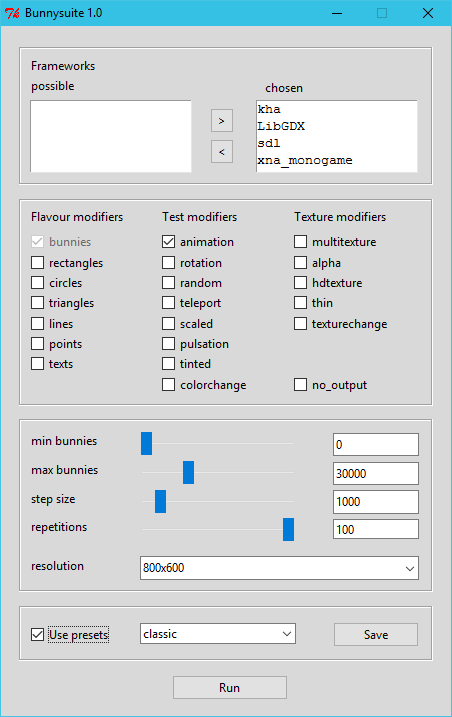
\includegraphics[width=0.7\textwidth]{gui}
\label{dia:gui}
\end{figure}

\begin{figure}[!tbp]
  \centering
  \subfloat[Unterschreiten von 56 FPS.]{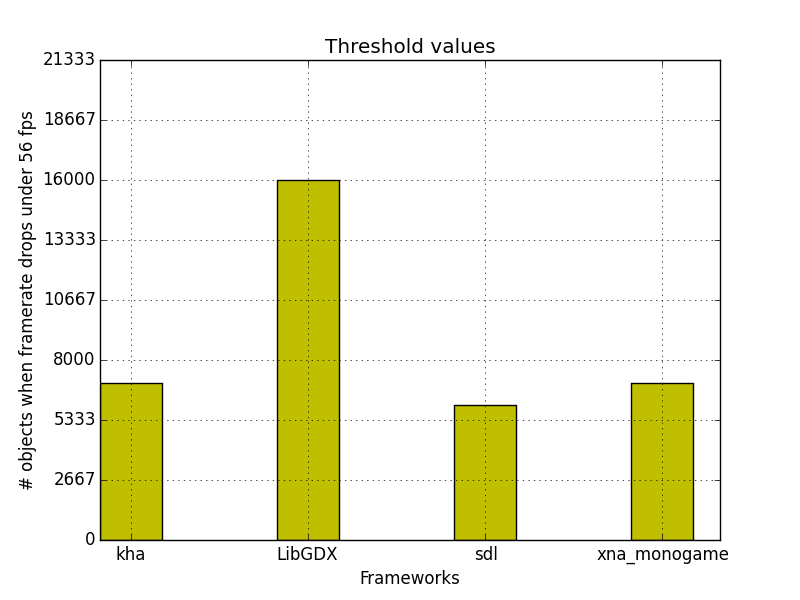
\includegraphics[width=0.4\textwidth]{bar_chart.png}\label{dia:bar}}
  \hfill
  \subfloat[Renderzeit pro Anzahl Objekte.]{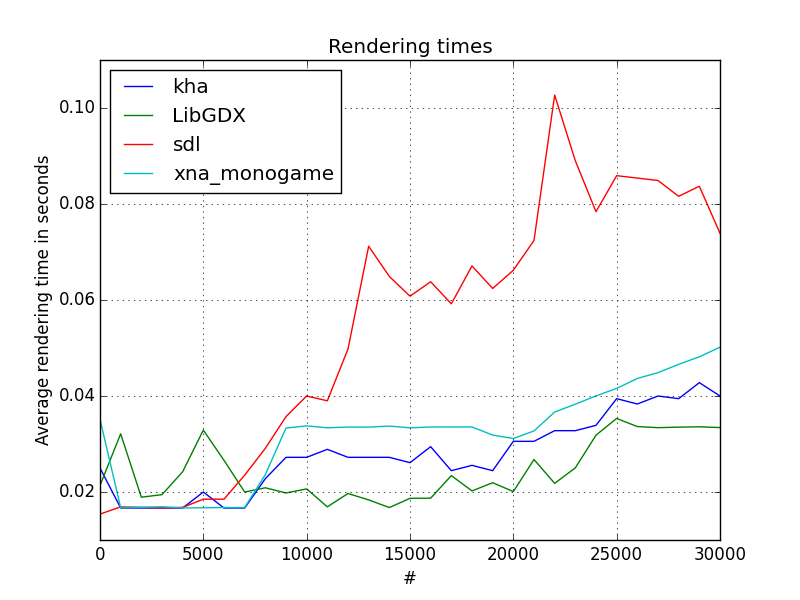
\includegraphics[width=0.4\textwidth]{line_graph.png}\label{dia:line}}
  \caption{Die generierten Diagramme.}
\end{figure}

\subsection{Tests direkt starten}
Tests können auch ohne GUI direkt gestartet werden. Dazu müssen die zu testenden Frameworks und die gewünschten Werte für die Parameter in die Datei \textit{run\_test.py} hineingeschrieben werden. Anschließend startet man dieses Skript. Der restliche Ablauf (Durchführung der Tests und Ausgabe des Diagramms) ist genauso wie bei der GUI, insbesondere werden auch die beiden Diagramme und der Report im Unterordner "results" erzeugt.

\chapter{Ergebnisse der Messungen}
\label{ch:results}
In diesem Kapitel stellen wir ein paar interessante Ergebnisse von Messungen vor, die wir mit den Frameworks durchgeführt haben.\\
Dazu nutzen wir die beiden Computersysteme, deren Eckdaten in Tabelle \ref{tab:allspecs} zu finden sind. Bei System 1 handelt es sich um ein günstiges Notebook, während System 2 ein typischer Gamer-PC ist.

\begin{table}
    \begin{tabular}{ | l | c | c |}
    \hline \\
    			& System 1						& System 2      						\\ \hline
    Modellname 	& Acer Aspire E1-531			& Custom-PC 							\\ \hline
    CPU 		& Intel Pentium 2020M (2,4 GHz) & Intel Xeon E3-1231 v3 @ 4 x 3.4 GHz 	\\ \hline
    GPU 		& Intel HD Graphics				& NVidia Geforce GTX 780				\\ \hline
    RAM 		& 4096 MB						& 16384 MB 								\\ \hline
    \end{tabular}
    \caption{Spezifikationen der beiden Testrechner}
   	\label{tab:allspecs}
\end{table}

\section{XNA Forced VSync?}
Diese Messung fand auf System 2 mit folgenden Parametern statt:
\begin{description}
\item[modifiers:] bunnies, random, pulsation
\item[frameworks:] kha, LibGDX, sdl, xna\_monogame
\item[minBunnies:] 0
\item[maxBunnies:] 100000
\item[stepSize:] 1000
\item[repetitions:] 10
\item[resolution:] 1280x720
\end{description}
Es wurden somit alle 10 Frames 1000 neue Bunnies mit Standardtextur an eine zufällige Position gezeichnet. Zusätzlich wurden alle Bunnies mit jedem Frame neu skaliert.\\ 
\begin{figure}
\caption{Ergebnis der XNA Forced VSync Messung}
\centering
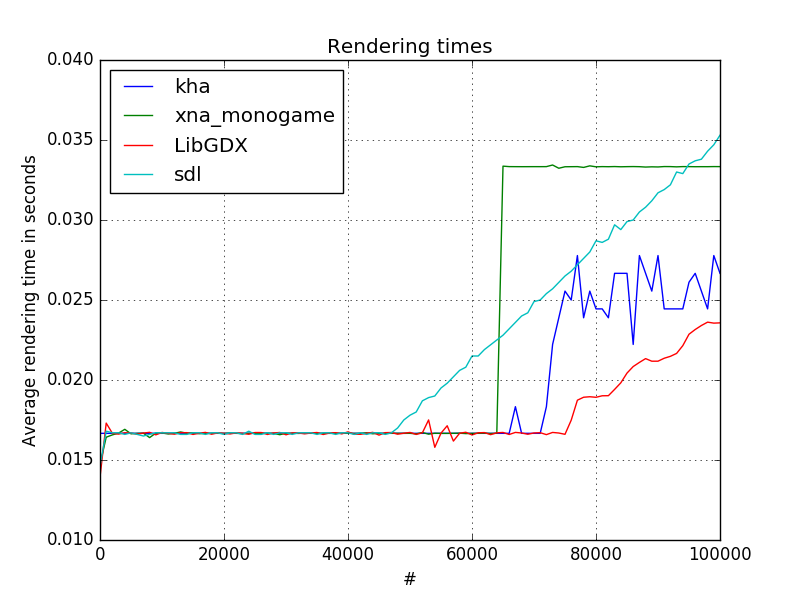
\includegraphics[width=0.8\textwidth]{xna_forced}
\label{dia:xna_forced}
\end{figure}
Diagramm \ref{dia:xna_forced} zeigt die Ergebnisse. Man sieht, dass XNA bei 62000 Bunnies in der Renderzeit plötzlich einen Sprung von 0,016s = 60fps zu 0,033s = 30fps vollzieht. SDL und LibGDX zeigen hier einen linearen Anstieg, so wie es erwartet wird. Kha macht um die 72000 Bunnies auch einen Sprung von 0,016s zu 0,025s = 40fps, und oszilliert anschließend um diesen Wert. Hier könnte Textur-Caching eine Rolle spielen. \\
Das abnormale Verhalten von XNA ist hier von besonderem Interesse. Mit diesem Testsetup lässt sich das Verhalten von XNA zuverlässig reproduzieren, tritt aber in anderen Setups nicht mehr auf. Stattdessen kommt es auch hier zu einem linearen Anstieg der Renderzeit (siehe Diagramm \ref{dia:xna_normal}).
\begin{figure}
\caption{Ergebnis Diagramm: Normales XNA Verhalten}
\centering
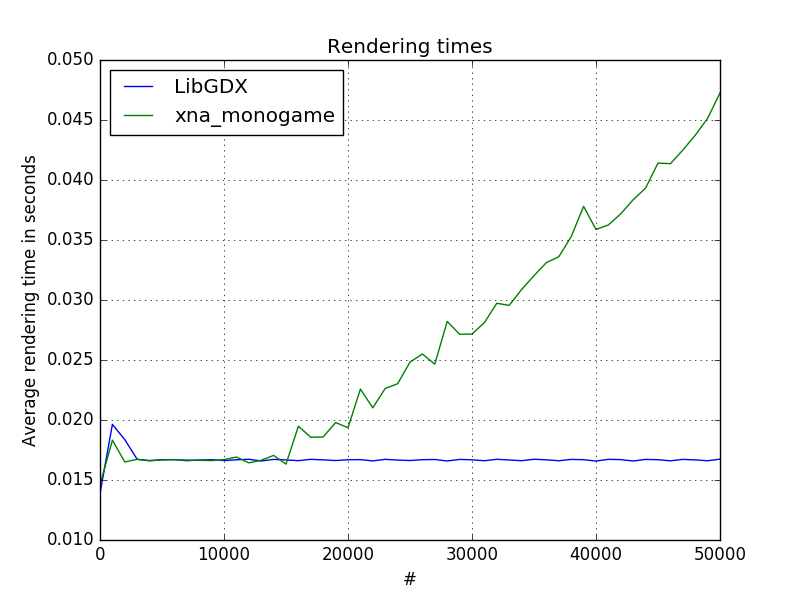
\includegraphics[width=0.8\textwidth]{xna_normal}
\label{dia:xna_normal}
\end{figure}
Da die Renderzeiten hier genau auf die übliche Bildwiederholungsrate von 60Hz passt, liegt die Vermutung nahe, dass es sich hier um aktiviertes VSync handelt, um Tearing zu verhindern. Dies tritt auf, wenn eine Ausgabe auf den Bildschirm erfolgen soll, die genau mit der Refresh-Phase VBlank des Monitors zusammenfällt. Um dies zu verhindern, wird die Ausgabe mit diesen Phasen synchronisiert. Diese Option ist aber bei der Implementierung der Tests im Framework explizit deaktiviert worden. Ebenso spricht das normale Verhalten in anderen Tests gegen diese These. \\
Eine abschließende Erklärung konnte nicht gefunden werden. 

\section{SDL Primitive}
Diese Messung fand auf System 2 mit folgenden Parametern statt:
\begin{description}
\item[modifiers:] rectangles, circles, triangles, lines, points, rotation, random, pulsation
\item[frameworks:] kha, LibGDX, sdl, xna\_monogame
\item[minBunnies:] 0
\item[maxBunnies:] 50000
\item[stepSize:] 1000
\item[repetitions:] 10
\item[resolution:] 1280x720
\end{description}
Es wurden somit alle 10 Frames 1000 zufällige Objekte der Primitive Dreieck, Rechteck, Kreis, Linie und Punkt an eine zufällige Screen-Position hinzugefügt. Jedes Objekt ändert mit jedem Frame seine Skalierung. Die Ergebnisse werden in Diagramm \ref{dia:sdl_primitives} dargestellt.
\begin{figure}
\caption{Ergebniss Diagramm der Primitiven Messung}
\centering
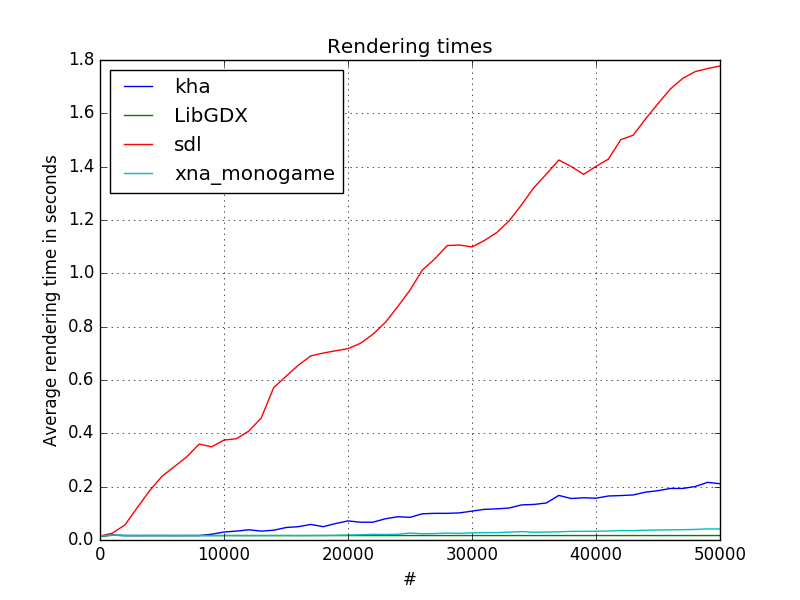
\includegraphics[width=0.8\textwidth]{sdl_primitives}
\label{dia:sdl_primitives}
\end{figure}
Bei der Darstellung und Skalierung von Primitiven hat SDL massive Probleme. Während die anderen Frameworks weit unter 1s Renderzeit bleiben, erreicht SDL bei 26000 Objekten eine Renderzeit von 1s, und erreicht gegen Ende 1,8s Renderzeit. Das ist 9 mal so lange wie das nächstlangsame Framework. SDL erreicht nie den Idealwert von 0,016s = 60fps Renderzeit und schon bei 2000 Objekten wird eine Renderzeit von 0,1s = 10fps erreicht. Die Ergebnisse zeigen, dass \textit{SDL2\_gfx}, das für das Rendering von Primitiven eingesetzt wurde, noch nicht besonders gut optimiert ist.\\

\chapter{Zusammenfassung und Ausblick}
Im Rahmen des Serious Games Praktikums wurde \textit{BunnySuite} entwickelt, ein Benchmark-Framework für 2D-Grafik-Libraries. Im Vergleich zu BunnyMark sind die Messungen von BunnySuite vollautomatisch und ohne Benutzerinteraktion durchführbar, außerdem sind die Testergebnisse detaillierter und werden dem Benutzer systematischer präsentiert. Es wurde eine Vielzahl von Testfällen (Rotation, Skalierung, Primitive, etc.) identifiziert, welche im Framework als Test-Modifier frei kombinierbar sind. Für die vier Bibliotheken Kha, LibGDX, SDL und XNA/Monogame wurden Implementierungen entwickelt. Bei der Entwicklung wurde vor allem auf eine hohe Vergleichbarkeit geachtet. Deshalb wurde der Effekt von allen Test-Modifiern genau definiert.\\
In dieser Ausarbeitung wurden außerdem einige Tests analysiert, die mit BunnySuite durchgeführt wurden. Dabei hat sich gezeigt, dass BunnySuite-Tests aufgrund ihrer Modularität gut dazu geeignet sind, Schwachstellen von Bibliotheken gezielt offenzulegen. 
\\
Als Future Work kann BunnySuite noch um weitere Frameworks erweitert werden. Insbesondere Frameworks für 2D-Grafik im Browser mit der Zielplattform HTML5 sollten auch im Browser ausgeführt werden und verglichen werden können. Hierbei besteht das Problem, dass man aus einem Browser heraus keine Logfiles anlegen kann, da ein Zugriff auf das lokale Dateisystem aus Sicherheitsgründen nicht möglich ist. Das könnte mit einem Automatisierungs-Tool wie Selenium\footnote{\url{http://www.seleniumhq.org/}} gelöst werden.\\
Außerdem können die Implementierungen für die vier Bibliotheken, insbesondere die für SDL, noch auf Optimierungspotential untersucht werden.
